\section{1174040 - Hagan Rowlenstino A. S}
    \subsection{Teori}
    \begin{enumerate}
        \item Why words need to be Vectorizer
        \subitem karena kata - kata yang digunakan untuk memproses data agar dapat menjadi bagian dati kumpulan data atatu atribut yang dapat dibaca oleh sistem machine learning karena sistem tersebut tidak dapat memproses data text secara langsung dan harus di convert terlebih dahulu kedalam bilangan.untuk ilustrasinya dapat dilihat pada gambar
        \begin{figure}[H]
            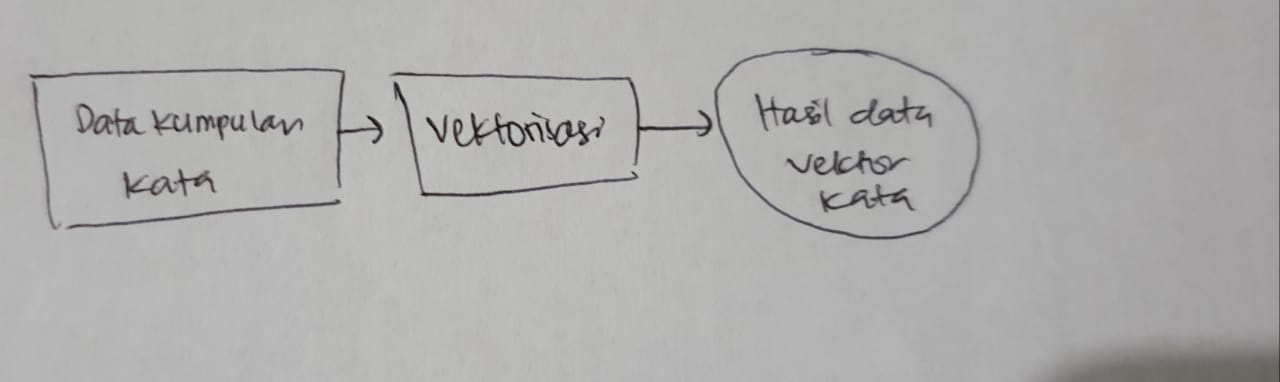
\includegraphics[width=4cm]{figures/1174040/chapter5/teori1.jpeg}
            \centering
            \caption{Vektorisasi Kata}
        \end{figure}
        
        \item Why Dimension of Google dataset can reach 300
        \subitem Dimensi dataset dari google bisa mencapai 300 karena dimensi dari vektor tersebut digunakan untuk membandingkan bobot dari setiap data kata yang diproses. ilustrasi dapat dilihat pada gambar
        \begin{figure}[H]
            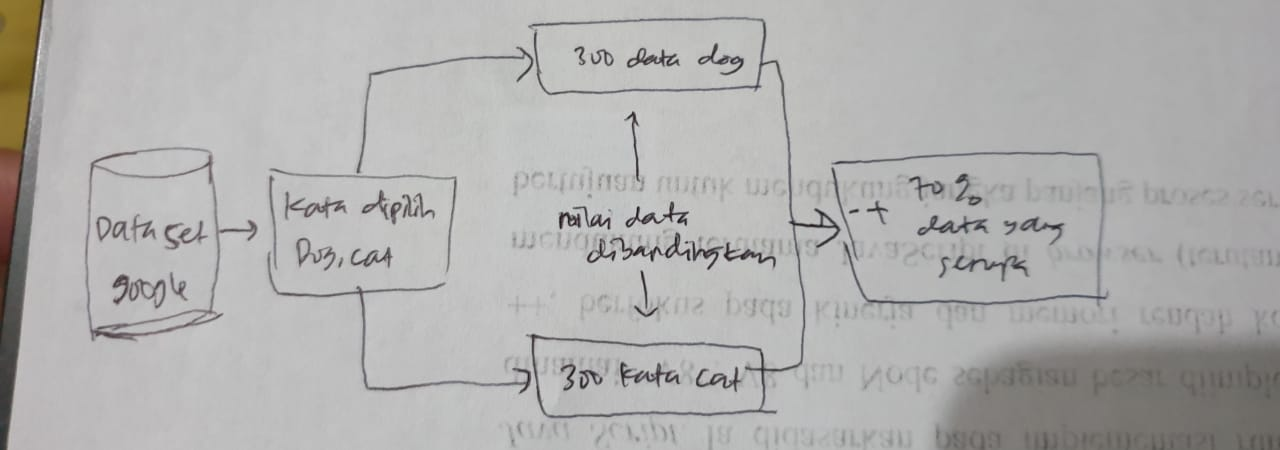
\includegraphics[width=4cm]{figures/1174040/chapter5/teori2.jpeg}
            \centering
            \caption{Dataset Google}
        \end{figure}
        
        \item Concept of Vectorizer on words
        \subitem pada vektorisasi dengan menggunakan Word2Vec memiliki kelebihan yang dapat dibedakan dengan pengguaan bag of words yang biasanya.  pada bag of word pemrosesan data tidak dapat menganalisa data yang memiliki makna sama namun penulisannya berbeda, namun pada penggunaan Word2Vec proses tersebut dapat berjalan dengan lebih mudah contohnya adalah penulisan kata please dengan plz. untuk ilustrasi datanya bisa dilihat dalam gambar
        \begin{figure}[H]
            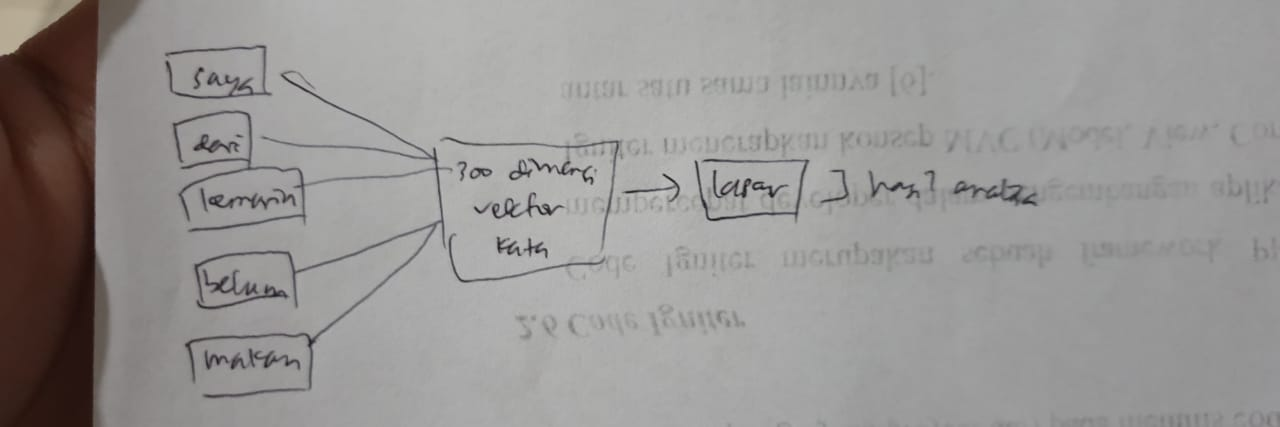
\includegraphics[width=4cm]{figures/1174040/chapter5/teori3.jpeg}
            \centering
            \caption{Concept of Vectorizer on words}
        \end{figure}
        
        \item Concept of Vectorizer on documents
        \subitem vektorisasi pada Doct2Vec dimana data yang terdapat pada file document tersebut diolah dengan melakukan pemrosesan yang mengutamakan nilai data filenamenya atau atribut utama dimana nilai data inputnya tidak terlalu diproses. ilustrasinya dapat dilihat pada gambar
        \begin{figure}[H]
            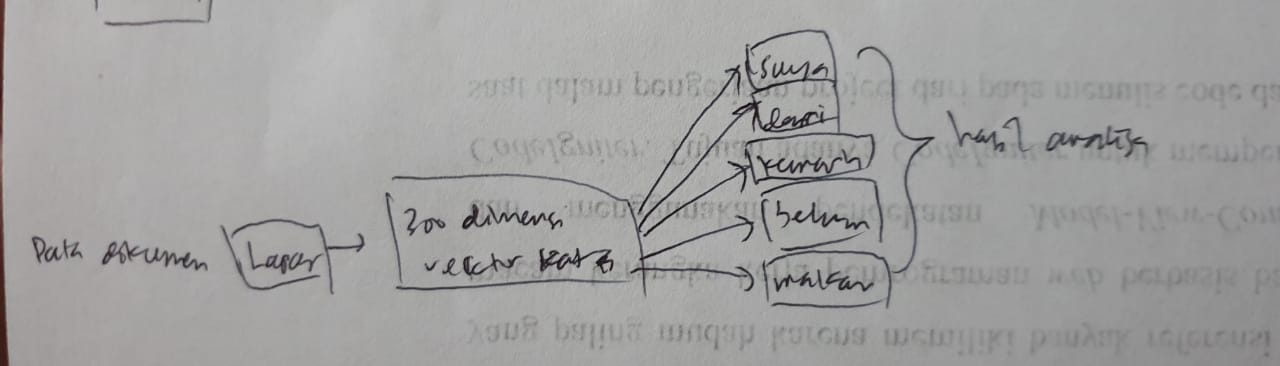
\includegraphics[width=4cm]{figures/1174040/chapter5/teori4.jpeg}
            \centering
            \caption{Concept of Vectorizer on Documents}
        \end{figure}
        
        \item What is mean and deviation standart
        \subitem Mean adalah nilai rata-rata dari beberapa buah data. Nilai mean dapat ditentukan dengan membagi jumlah data dengan banyaknya data.
        
        \subitem Standar deviasi adalah nilai statistik yang digunakan untuk menentukan bagaimana sebaran data dalam sampel, dan seberapa dekat titik data individu ke mean – atau rata-rata – nilai sampel.
        
        untuk ilustrasi data mean dan deviation standart bisa dilihat pada gambar
        \begin{figure}[H]
            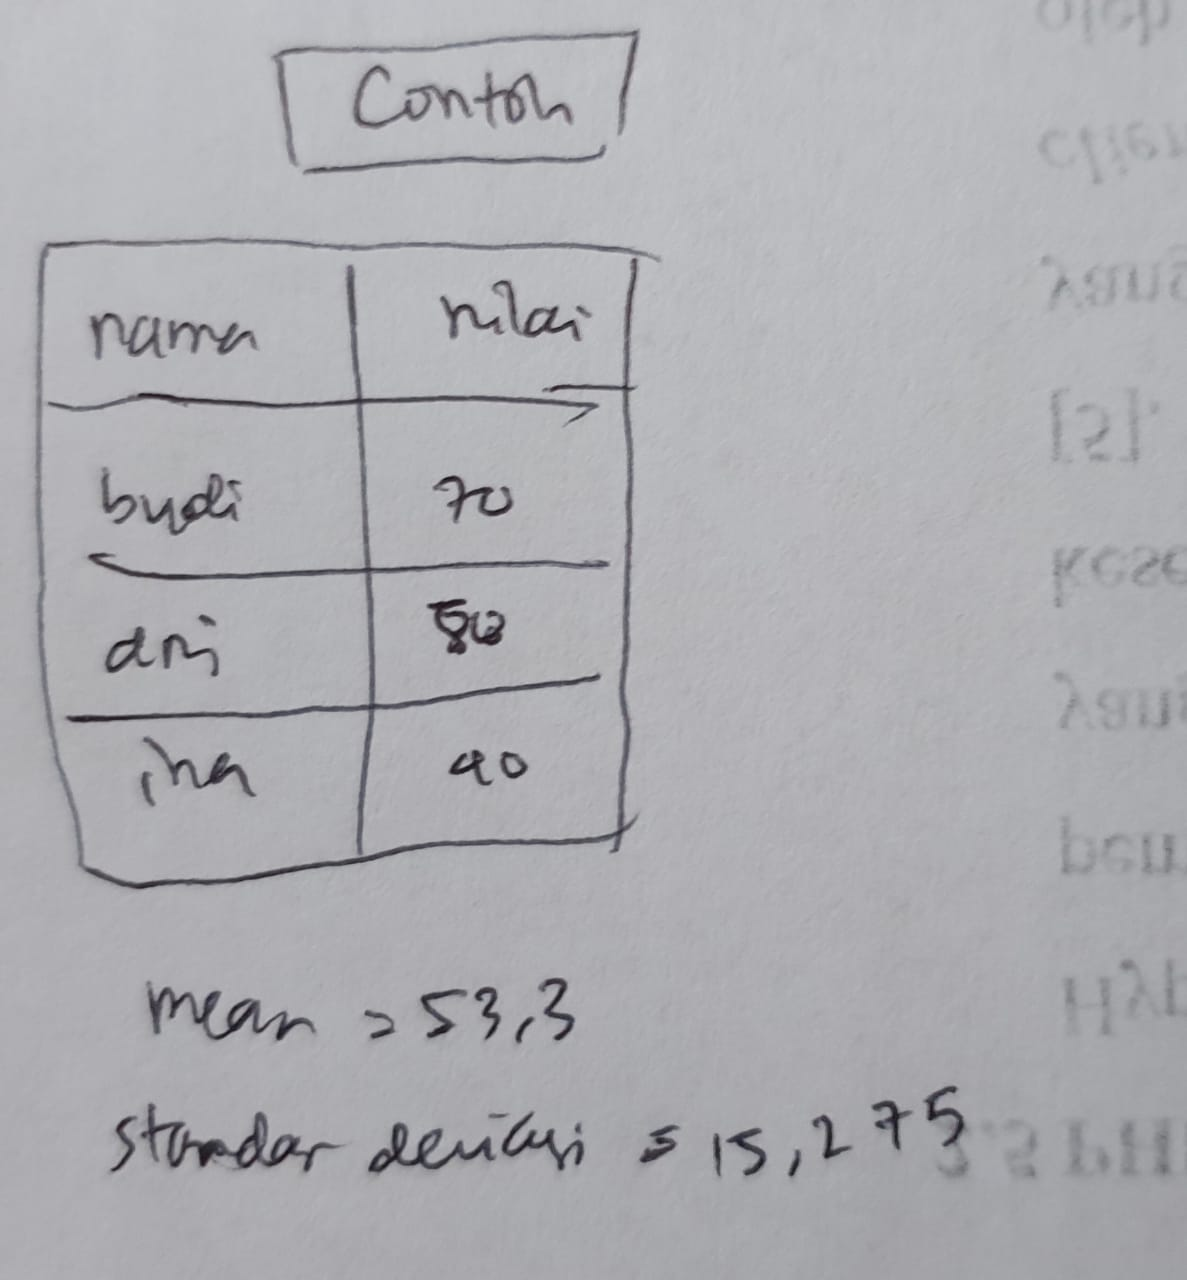
\includegraphics[width=4cm]{figures/1174040/chapter5/teori5.jpeg}
            \centering
            \caption{Mean and Deviation Standard}
        \end{figure}
        
        \item What is skip-gram
        \subitem Skip-gram merupakan teknik yang digunakan di area speech processing, dimana n-gram yang dibentuk kemudian ditambahkan juga dengan tindakan “skip” pada token-tokennya. contohnya terdapat pada gambar
        \begin{figure}[H]
            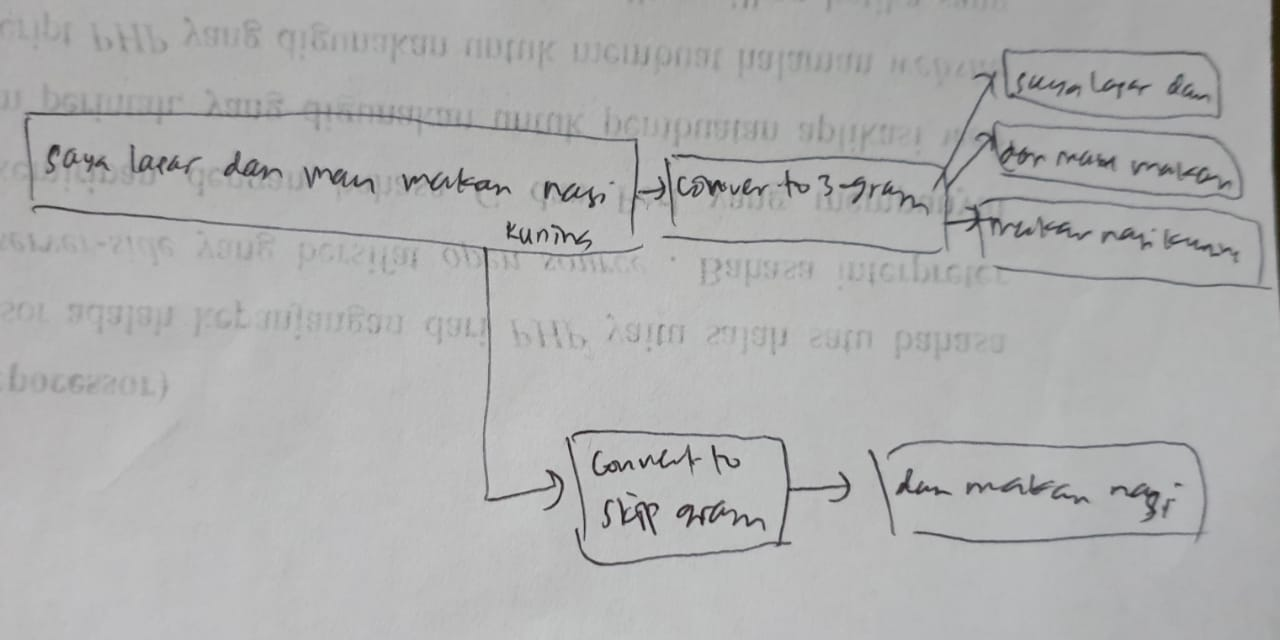
\includegraphics[width=4cm]{figures/1174040/chapter5/teori6.jpeg}
            \centering
            \caption{Skip-Gram}
        \end{figure}
    \end{enumerate}
    \subsection{Praktek}
        \begin{enumerate}
        \item Try datasets GoogleNews-vectors
        \begin{itemize}
        \item berikut adalah hasil dari code yang digunakan untuk memanggil data library GENSIM dengan menggunakan perintah import, lalu dari library tersebut diambillah data yang akan digunakan untuk memproses data dari GoogleNews-vector. ilustrasi dapat dilihat pada gambar
        \begin{figure}[H]
            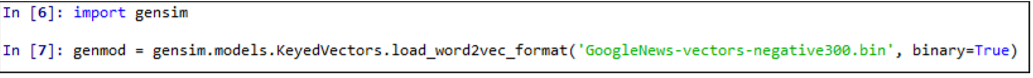
\includegraphics[width=4cm]{figures/1174040/chapter5/1.png}
            \centering
            \caption{import gensim dan olah data GoogleNews-vector}
        \end{figure}
        
        \item lalu pada penggunaan code berikut ini akan mengolah data LOVE yang terdapat pada file GoogleNews-vector, hasil dari pemrosesannya dapat dilihat pada gambar
        \begin{figure}[H]
            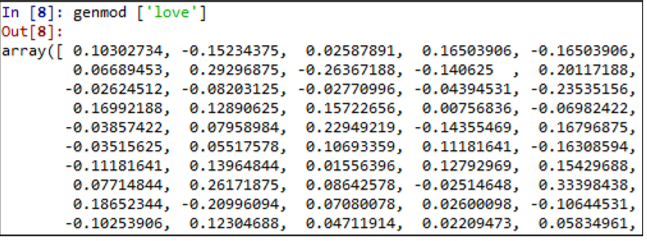
\includegraphics[width=4cm]{figures/1174040/chapter5/2.png}
            \centering
            \caption{hasil olah data LOVE pada GoogleNews-vector}
        \end{figure}
        
        \item  lalu pada penggunaan code berikut ini akan mengolah data FAITH yang terdapat pada file GoogleNews-vector, hasil dari pemrosesannya dapat dilihat pada gambar
        \begin{figure}[H]
            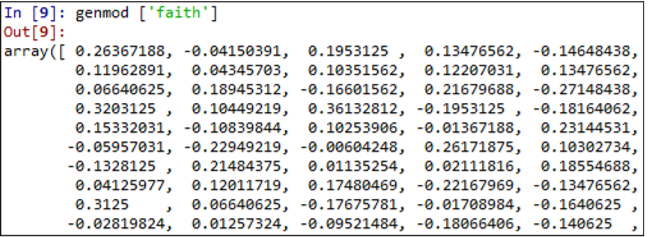
\includegraphics[width=4cm]{figures/1174040/chapter5/3.png}
            \centering
            \caption{hasil olah data FAITH pada GoogleNews-vector}
        \end{figure}
        
        \item  lalu pada penggunaan code berikut ini akan mengolah data FALL yang terdapat pada file GoogleNews-vector, hasil dari pemrosesannya dapat dilihat pada gambar
        \begin{figure}[H]
            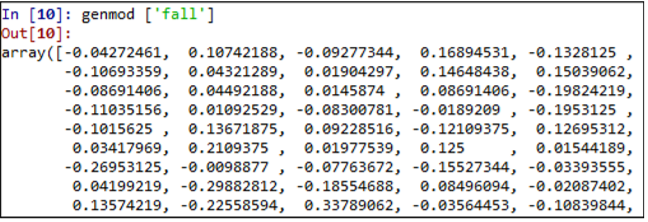
\includegraphics[width=4cm]{figures/1174040/chapter5/4.png}
            \centering
            \caption{hasil olah data FALL pada GoogleNews-vector}
        \end{figure}
        
        \item  lalu pada penggunaan code berikut ini akan mengolah data SICK yang terdapat pada file GoogleNews-vector, hasil dari pemrosesannya dapat dilihat pada gambar
        \begin{figure}[H]
            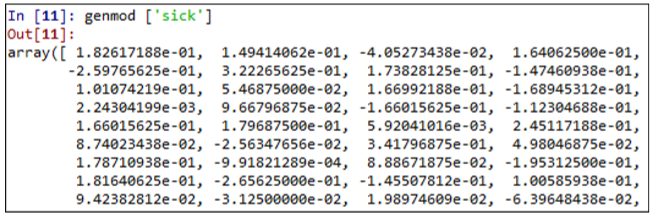
\includegraphics[width=4cm]{figures/1174040/chapter5/5.png}
            \centering
            \caption{hasil olah data SICK pada GoogleNews-vector}
        \end{figure}
        
        \item  lalu pada penggunaan code berikut ini akan mengolah data CLEAR yang terdapat pada file GoogleNews-vector, hasil dari pemrosesannya dapat dilihat pada gambar
        \begin{figure}[H]
            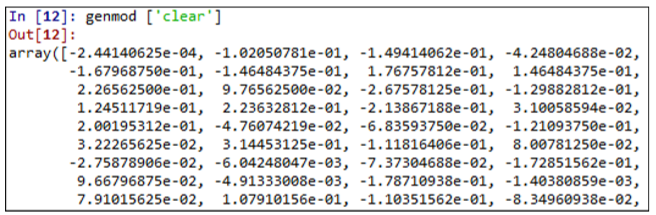
\includegraphics[width=4cm]{figures/1174040/chapter5/6.png}
            \centering
            \caption{hasil olah data CLEAR pada GoogleNews-vector}
        \end{figure}
        
        \item  lalu pada penggunaan code berikut ini akan mengolah data SHINE yang terdapat pada file GoogleNews-vector, hasil dari pemrosesannya dapat dilihat pada gambar
        \begin{figure}[H]
            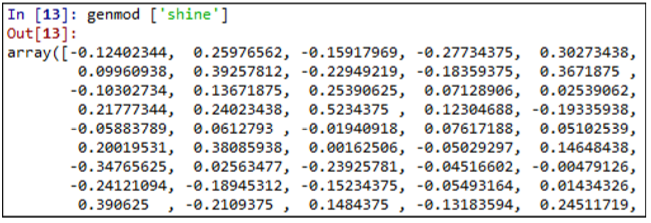
\includegraphics[width=4cm]{figures/1174040/chapter5/7.png}
            \centering
            \caption{hasil olah data SHINE pada GoogleNews-vector}
        \end{figure}
        
        \item  lalu pada penggunaan code berikut ini akan mengolah data BAG yang terdapat pada file GoogleNews-vector, hasil dari pemrosesannya dapat dilihat pada gambar
        \begin{figure}[H]
            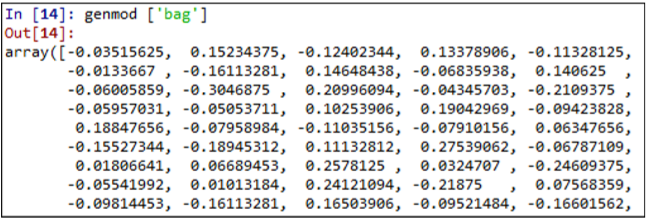
\includegraphics[width=4cm]{figures/1174040/chapter5/8.png}
            \centering
            \caption{hasil olah data BAG pada GoogleNews-vector}
        \end{figure}
        
        \item  lalu pada penggunaan code berikut ini akan mengolah data CAR yang terdapat pada file GoogleNews-vector, hasil dari pemrosesannya dapat dilihat pada gambar
        \begin{figure}[H]
            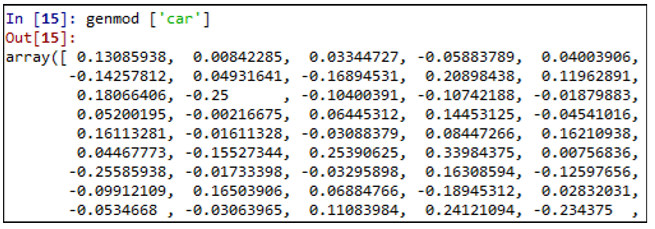
\includegraphics[width=4cm]{figures/1174040/chapter5/9.png}
            \centering
            \caption{hasil olah data CAR pada GoogleNews-vector}
        \end{figure}
        
        \item  lalu pada penggunaan code berikut ini akan mengolah data WASH yang terdapat pada file GoogleNews-vector, hasil dari pemrosesannya dapat dilihat pada gambar
        \begin{figure}[H]
            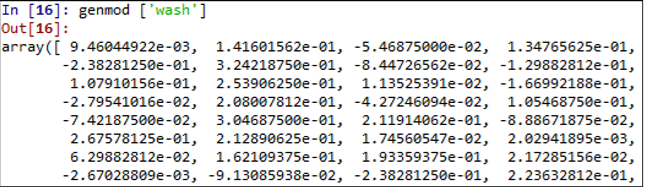
\includegraphics[width=4cm]{figures/1174040/chapter5/10.png}
            \centering
            \caption{hasil olah data WASH pada GoogleNews-vector}
        \end{figure}
        
        \item  lalu pada penggunaan code berikut ini akan mengolah data MOTOR yang terdapat pada file GoogleNews-vector, hasil dari pemrosesannya dapat dilihat pada gambar 
        \begin{figure}[H]
            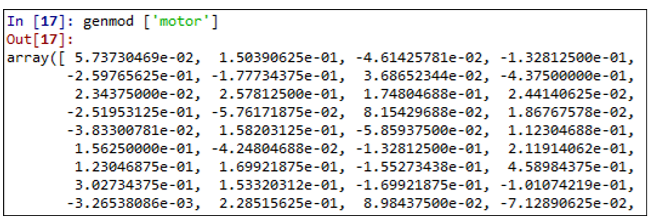
\includegraphics[width=4cm]{figures/1174040/chapter5/11.png}
            \centering
            \caption{hasil olah data MOTOR pada GoogleNews-vector}
        \end{figure}
        
        \item  lalu pada penggunaan code berikut ini akan mengolah data CYCLE yang terdapat pada file GoogleNews-vector, hasil dari pemrosesannya dapat dilihat pada gambar
        \begin{figure}[H]
            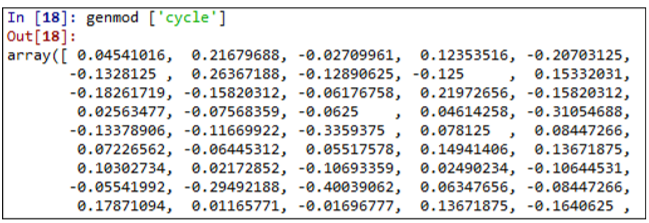
\includegraphics[width=4cm]{figures/1174040/chapter5/12.png}
            \centering
            \caption{hasil olah data CYCLE pada GoogleNews-vector}
        \end{figure}
        
        \item  dan pada hasil code berikut ini adalah hasil dari proses penggunaan perintah code similarity yang akan menghitung nilai value data yang dibandingkan dengan masing - masing kata seperti pada hasil dari perbandingan kata LOVE disandingkan dengan FAITH menghasilkan nilai 37 persen, sedangkan kata WASH dan SHINE menghasilkan nilai 27 persen dan kata CAR yang disandingkan dengan kata MOTOR menghasilkan 48 persen, dimana kita dapat menyimpulkan bahwa semakin data kata tersebut memiliki tingkat kesamaan yang tinggi maka nilai hasil yang ditampilkanpun akan semakin tinggi. ilustrasi bisa dilihat pada gambar
        \begin{figure}[H]
            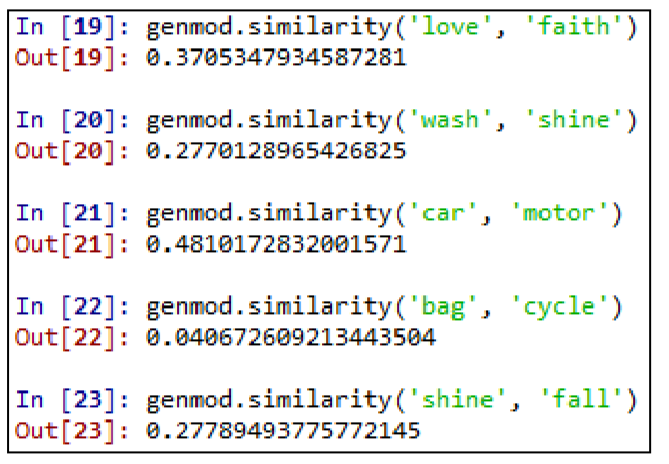
\includegraphics[width=4cm]{figures/1174040/chapter5/13.png}
            \centering
            \caption{hasil olah data  pada GoogleNews-vector menggunakan SIMILARITY}
        \end{figure}
        \end{itemize}
        
        \item extract\_words dan PermutedSentences
        \subitem pada penjelasan berikut ini akan menyangkut pembersihan data yang akan digunakan untuk diproses, dimana data akan di EXTRACT dari setiap katanya agar terbebas dari data TAG HTML, APOSTROPHES, TANDA BACA, dan SPASI yang berlebih. dengan menggunakan perintah code STRIP dan SPLIT. lalu penggunaan library random yang akan dibuat untuk melakukan KOCLOK data dengan acuan datanya adalah data yang terdapat pada variable KATA. untuk ilustrasi hasil dari codenya dapat dilihat pada gambar
        \begin{figure}[H]
            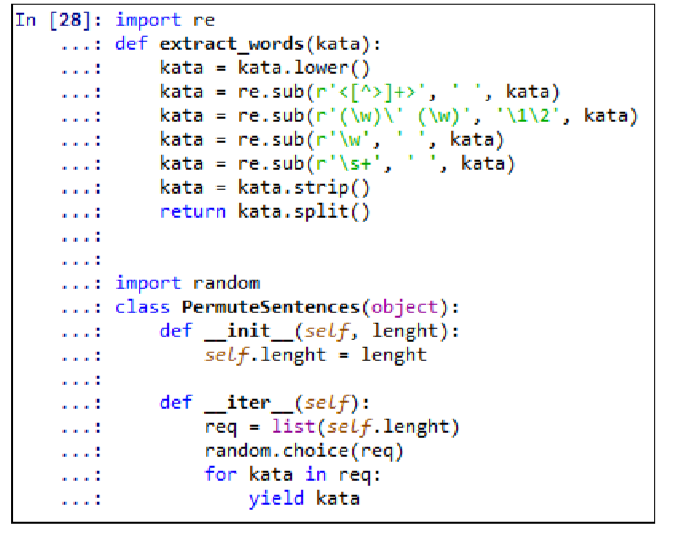
\includegraphics[width=4cm]{figures/1174040/chapter5/14.png}
            \centering
            \caption{hasil olah data  pada GoogleNews-vector menggunakan extract\_words dan PermuteSentences}
        \end{figure}
        
        \item TaggedDocument dan Doc2Vec
        \subitem gensim merupakan open-source model ruang vektor dan toolkit topic modeling, yang diimplementasikan dalam bahasa pemrograman Python. Untuk kinerja Gensim, digunakan NumPy, SciPy dan Cython (opsional). Gensim secara khusus ditujukan untuk menangani koleksi teks besar dengan menggunakan algoritma secara online. Gensim mengimplementasikan tf-idf, latent semantic analysis (LSA), Latent Dirichlet Analysis (LDA), dan lain-lain. 
        \subitem tagged document merupakan sebuah class yang terdapat pada pemrosesan data pada library gensim yang akan mengolah data teks yang ada pada dokumen - dokumen yang dipakai.
        \subitem Doc2Vec merupakan algoritma doct embedding, yaitu pemetaan dari dokumen menjadi vektor, serta pemetaan data dokumen 1 dan dokumen lainnya.
        ilustrasi dari tagged document dan Word2Vec ada pada gambar
        \begin{figure}[H]
            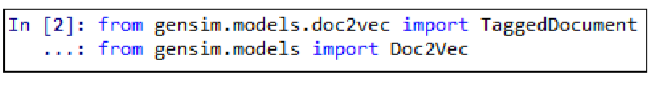
\includegraphics[width=4cm]{figures/1174040/chapter5/15.png}
            \centering
            \caption{TaggedDocument dan Doc2Vec}
        \end{figure}
        
        \item Praktek data training
        \subitem pertama buka data training yang akan diolah pada aplikasi python, import library OS dan membuat data variable unsup\_senteces dengan nilai array kosong. buatkan data direktori untuk memanggil data yang akan diolah dan buatkan juga variable data nilai fname yang akan memproses data dirname untuk diisikan pada variable unsup\_sentences. code yang digunakan dapat dilihat pada gambar
        \begin{figure}[H]
            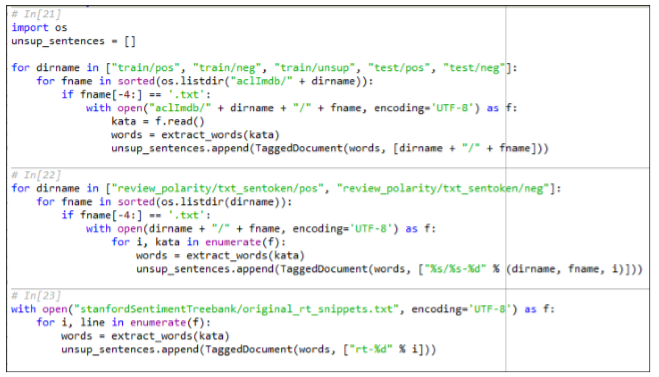
\includegraphics[width=4cm]{figures/1174040/chapter5/16.png}
            \centering
            \caption{data code praktek data training}
        \end{figure}
        
        data pada hasil code digambar berikut \ref{l1}, menghasilkan data pada gambar \ref{l2} yang akan memunculkan data variable DIRNAME, FNAME, KATA dan unsup\_sentences yang memiliki data sebanyak 55 kata dalam file yang diolah tersebut. hasil run dengan menggunakan code pada gambar \ref{l3}, menghasilkan data nilai yang terdapat pada gambar \ref{l4}. lalu pada code yang terdapat digambar \ref{l5}, menghasilkan data \ref{l6}.
        \begin{figure}[H]
            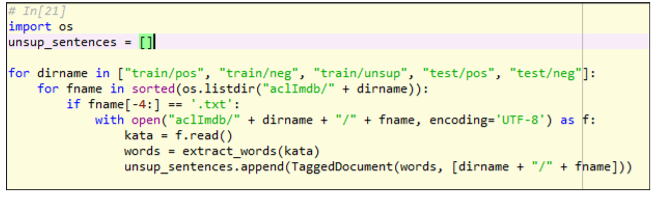
\includegraphics[width=4cm]{figures/1174040/chapter5/17.png}
            \centering
            \caption{data code praktek data training }
            \label{l1}
        \end{figure}
        \begin{figure}[H]
            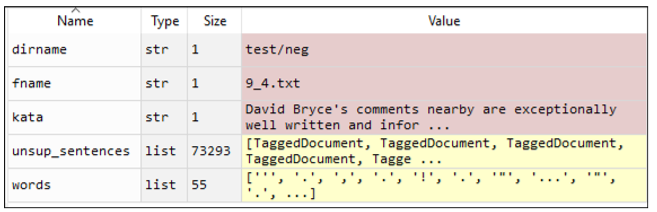
\includegraphics[width=4cm]{figures/1174040/chapter5/18.png}
            \centering
            \caption{data code praktek data training }
            \label{l2}
        \end{figure}
        \begin{figure}[H]
            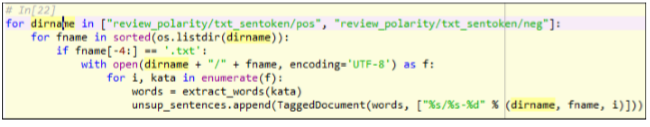
\includegraphics[width=4cm]{figures/1174040/chapter5/19.png}
            \centering
            \caption{data code praktek data training }
            \label{l3}
        \end{figure}
        \begin{figure}[H]
            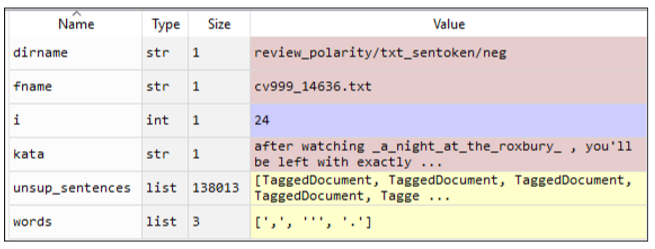
\includegraphics[width=4cm]{figures/1174040/chapter5/20.png}
            \centering
            \caption{data code praktek data training }
            \label{l4}
        \end{figure}
        \begin{figure}[H]
            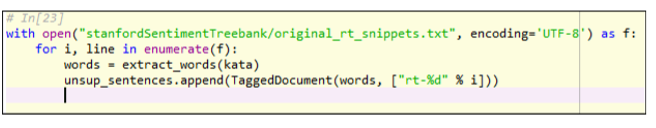
\includegraphics[width=4cm]{figures/1174040/chapter5/21.png}
            \centering
            \caption{data code praktek data training }
            \label{l5}
        \end{figure}
        \begin{figure}[H]
            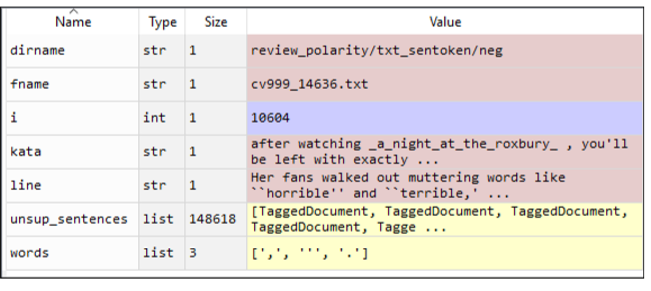
\includegraphics[width=4cm]{figures/1174040/chapter5/22.png}
            \centering
            \caption{data code praktek data training }
            \label{l6}
        \end{figure}
        
        \item Why need Shuffled and Clean memory
        \subitem dilakukan shuffled adalah agar datanya lebih mudah untuk diolah dan untuk menentukan tingkat tinggi akurasi dari hasil pemrosesan. dan dilakukan pembersihan memory adalah agar chace yang disimpan tidak membuat proses pada komputer mejadi lambat dan dapat digunakan untuk memproses data lainnya agar menjadi lebih ringan dan cepat.
        pada gambar \ref{l7} adlah proses untuk melakukan pengoclokan data dan pada gambar \ref{l8} adalah proses untuk memasukan data unsup\_sentences kedalam variable muter untuk diproses dengan class PermuterSentences. dan pada gambar \ref{l9} adalah code yang digunakan untuk membersihkan data memory.
        \begin{figure}[H]
            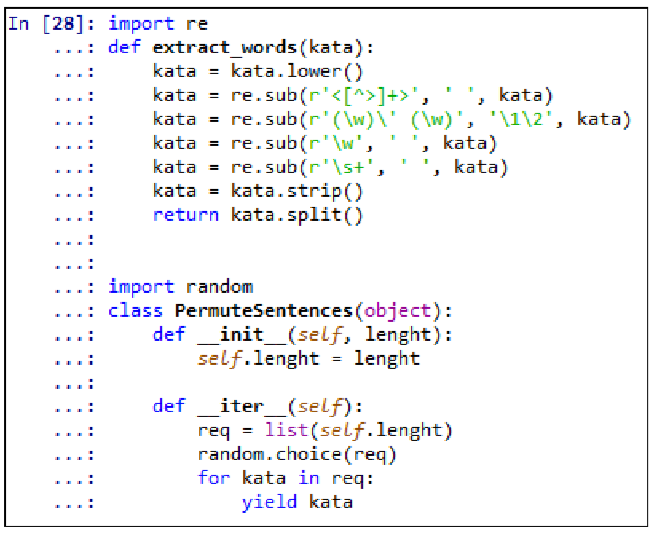
\includegraphics[width=4cm]{figures/1174040/chapter5/23.png}
            \centering
            \caption{Shuffled dan Randomisasi data }
            \label{l7}
        \end{figure}
        \begin{figure}[H]
            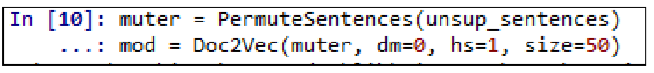
\includegraphics[width=4cm]{figures/1174040/chapter5/24.png}
            \centering
            \caption{pembuatan variable muter untuk memuat data unsup\_sentences}
            \label{l8}
        \end{figure}
        \begin{figure}[H]
            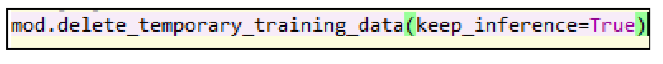
\includegraphics[width=4cm]{figures/1174040/chapter5/25.png}
            \centering
            \caption{code untuk membersihkan data memory}
            \label{l9}
        \end{figure}
        
        
        \item Why model have to be saved
        \subitem dalam pengolahan data dengan menggunakan proses yang panjang ditakutkan data yang sudah diproses tersebut dapat hilang jika terdapat kejadian atau emergency pada saat pengolahan dan pemrosesan data, misalnya harddisk error atau pun listrik yang padam. dan proses penyimpanan data juga dilakukan agar data yang sudah diolah data dipanggil lagi tanpa harus melakukan proses dari awal sehingga tidak memakan waktu. untuk code yang digunakan dapat dilihat pada gambar
        
        \begin{figure}[H]
            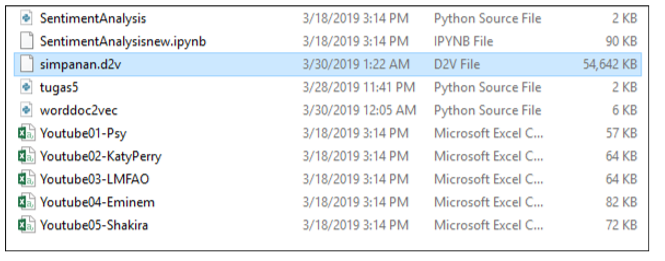
\includegraphics[width=4cm]{figures/1174040/chapter5/27.png}
            \centering
            \caption{data code save data}
        \end{figure}
        
        berikut ini adalah hasil file dari penggunaan code save tersebut. bisa dilihat pada gambar
        \begin{figure}[H]
            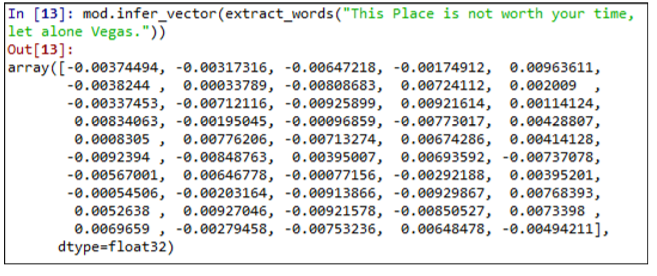
\includegraphics[width=4cm]{figures/1174040/chapter5/28.png}
            \centering
            \caption{hasil file simpan}
        \end{figure}
        
        \item infer\_vector
        \subitem berfungsi untuk dokumen baru, dan  bisa menggunakan data vektor yang dilatih secara massal, seperti yang disimpan dalam model, untuk dokumen yang merupakan bagian dari data training. untuk percobaannya dapat dilihat pada gambar
        \begin{figure}[H]
            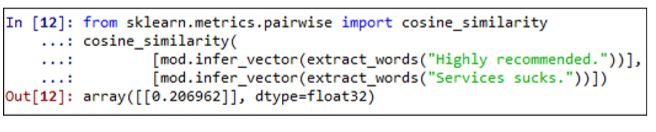
\includegraphics[width=4cm]{figures/1174040/chapter5/29.png}
            \centering
            \caption{code dan hasil infer\_vector}
        \end{figure}
        
        \item cosine\_similarity
        \subitem merupakan sebuah algoritma yang digunakan untuk membandingkan dari dua buah data yang bukan merupakan data vector untuk menguji nilai kemiripan data satu dengan data lainnya. hasil dari percobaan pada tugas no 8 ini dapat dilihat pada gambar \ref{l10} yang menghasilkan nilai akurasi sebesar 20 persen dan gambar \ref{l11} yang menghasilkan nilai akurasi sebesar 91 persen.
        \begin{figure}[H]
            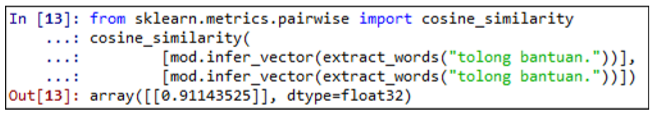
\includegraphics[width=4cm]{figures/1174040/chapter5/30.png}
            \centering
            \caption{code dan hasil penggunaan cosine\_similarity}
            \label{l10}
        \end{figure}
        
        \begin{figure}[H]
            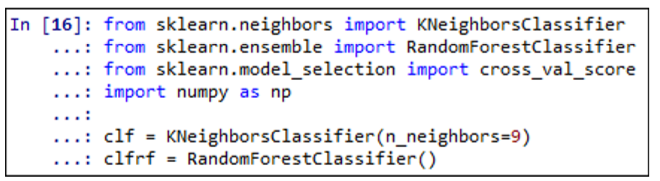
\includegraphics[width=4cm]{figures/1174040/chapter5/31.png}
            \centering
            \caption{code dan hasil penggunaan cosine\_similarity}
            \label{l11}
        \end{figure}
        
        \item Cross Validation
        \subitem pertama melakukan import data dari library KNeighborsClassifier, RandomForestClassifier, cross\_val\_score dan numpy yang digunakan untuk membuat data cross validasi dapat dilihat pada gambar
        \begin{figure}[H]
            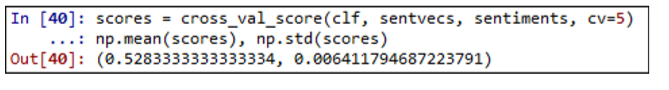
\includegraphics[width=4cm]{figures/1174040/chapter5/32.png}
            \centering
            \caption{memasukan code import library}
        \end{figure}
        
        \subitem lalu selanjutnya membuat data variable scores yang akan memuat nilai cross\_val\_score dengan datanya diambil dari KNeighborsClassifier yang terdiri dari sentvecs, sentiments dan clf dan mengolahnya menggunakan numpy untuk menampilkan data pada gambar yang menghasilkan nilai akurasi sebesar 53 persen.
        \begin{figure}[H]
            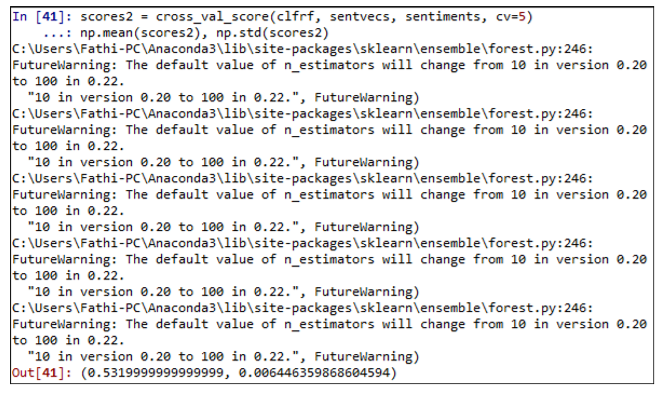
\includegraphics[width=4cm]{figures/1174040/chapter5/33.png}
            \centering
            \caption{perhitungan data KNeighborsClassifier dengan cross validasi}
        \end{figure}
        
        \subitem membuat data variable scores yang akan memuat nilai cross\_val\_score dengan datanya diambil dari RandomForestClassifier yang terdiri dari sentvecs, sentiments dan clfrf dan mengolahnya menggunakan numpy untuk menampilkan data pada gambar yang menghasilkan nilai akurasi sebesar 53 persen. 
        \begin{figure}[H]
            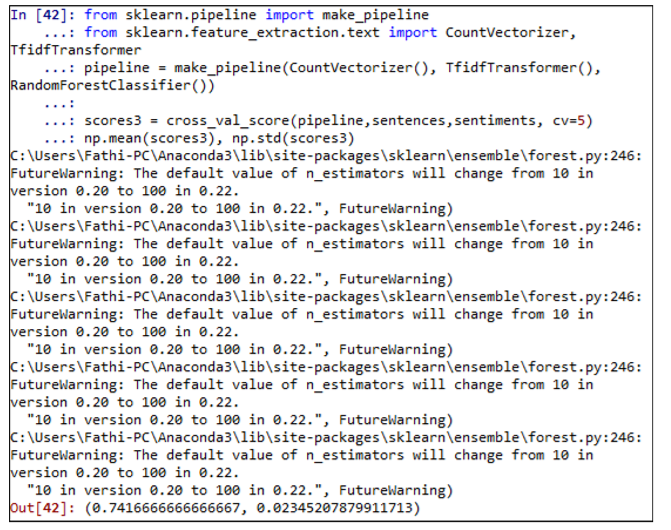
\includegraphics[width=4cm]{figures/1174040/chapter5/34.png}
            \centering
            \caption{perhitungan data  RandomForestClassifier dengan cross validasi}
        \end{figure}
        
        \subitem penggunaan make\_pipeline adalah untuk membuat data dari KNeighborsClassifier, RandomForestClassifier dan Vectorizer digabungkan untuk menghasilkan data nilai pada gambar menghasilkan nilai akurasi sebesar 74 persen. 
        \begin{figure}[H]
            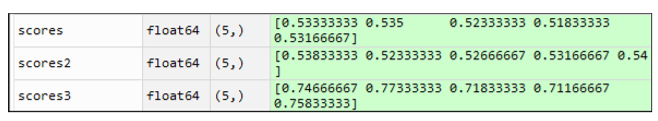
\includegraphics[width=4cm]{figures/1174040/chapter5/35.png}
            \centering
            \caption{perhitungan data Cross Validasi untuk nilai keseluruhan dari KNeighborsClassifier, RandomForestClassifier dan Vectorizer}
        \end{figure}
        
        \end{enumerate}